\subsection{Library}
\label{subsec:bcoollib}

Libraries are used to gather predefined event expressions and relations that can be imported by a \bcool specification (\emph{ImportedLibStatement} in Figure~\ref{fig:bcool}). \bcool relies on \moccml~\cite{moccmlbib} to define libraries of constraints between events. In this subsection, we overview the notion of \moccml library.

A \moccml library (\emph{RelationLibrary} in Figure~\ref{fig:moccml}) is a set of declarations together with their formal parameters. It also contains some definitions, which give the actual behavior of the declarations. There are two categories of constraint definitions: the \emph{Declarative Definitions} and the \emph{Constraint Automata Definitions}. A declarative definition is defined as a set of constraint instances. For more details, we refer the reader to~\cite{moccmloperbib} that described the declarative part inspired from the \ccsl language. A Constraint Automata Definition gives state based support for the definition of relations. This helps a language integrator in the definition of coordination protocols that may be complex like, for instance, the AMBA protocol~\cite{ambabus}. 

\begin{figure}[h]
	\center
	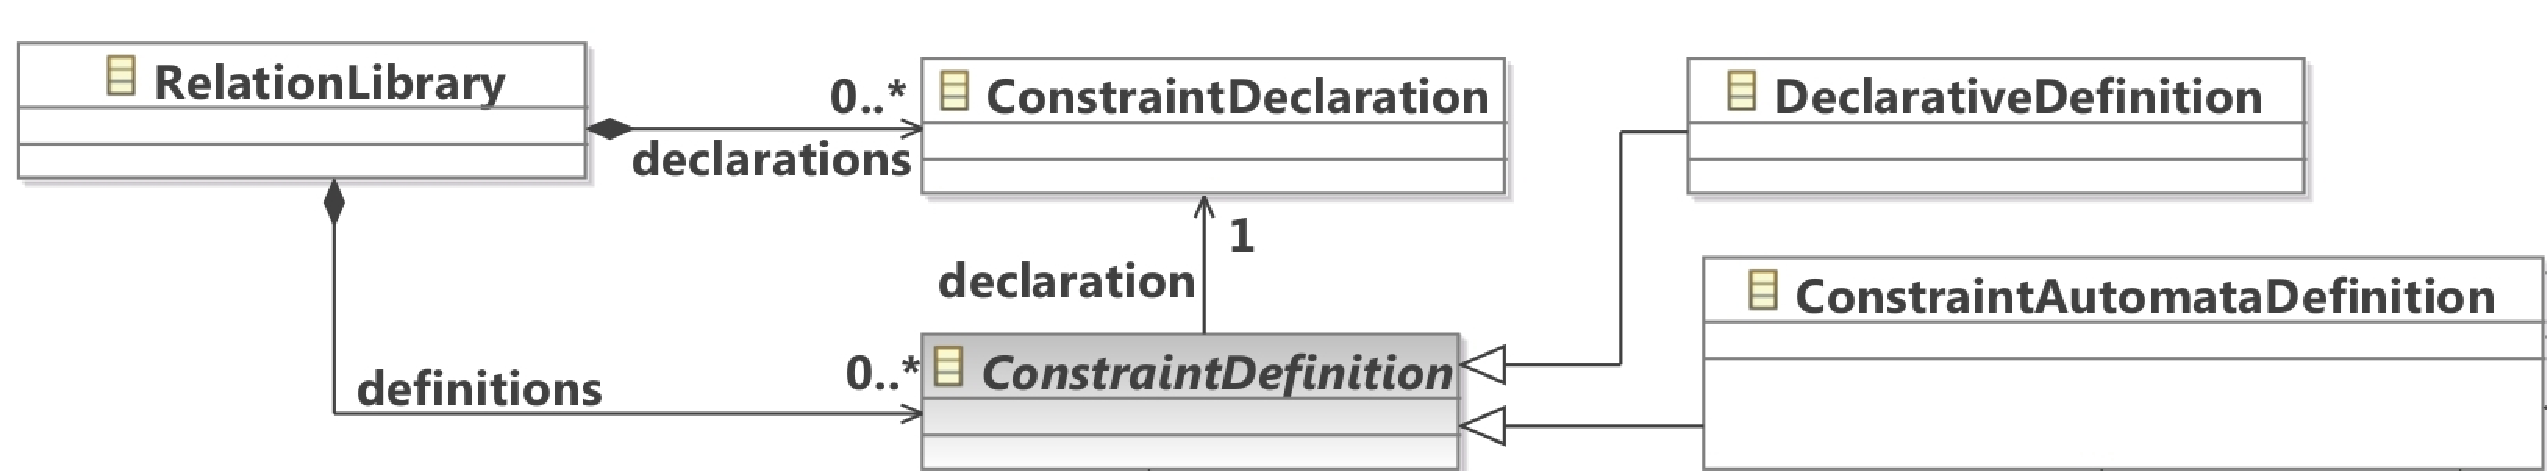
\includegraphics[width=.8\textwidth]{bcool/figs/moccmlmm}
	\caption{Excerpt of MoCCML Metamodel}
	\label{fig:moccml}
\end{figure}


To illustrate the use of \moccml for the definition of event relations, we propose to rewrite the coordination rule presented in Listing~\ref{lst:bcoolrunningexampletimed} by using an automata relation named \emph{RendezvousWithGlobalClock}. The relation accepts three events as parameters: \emph{sampled}, \emph{trigger} and \emph{executeIt}. The \emph{sampled} event identifies the event that will be sampled by the \emph{trigger}. The \emph{executeIt} event identifies the event that will be forced to occur simultaneously with the last sample of the \emph{sampled} event. The automata representation is made of two states: \emph{waitSampled} and \emph{waitTrigger} (see Figure~\ref{fig:moccmllib}). In \emph{waitSampled}, the event \emph{trigger} and \emph{sampled} are both allowed to tick but not the \emph{executeIt} event. When the event \emph{sampled} happens, such occurrence will be sampled by the next occurrence of the event \emph{trigger}. This is represented by the transition from \emph{waitSampled} to \emph{waitTrigger}. In this state, the event \emph{trigger} and \emph{executeIt} are forced to happen simultaneously. This represents the sampling of the last occurrence of the \emph{sampled} event. Conversely, in this state, the event \emph{sampled} is forbidden to occur~\footnote{For this example, we chose to forbid the occurrences of the \emph{sampled} event in the WaitTrigger state to prevent missing samples.}. 

\begin{figure}[h]
	\center
	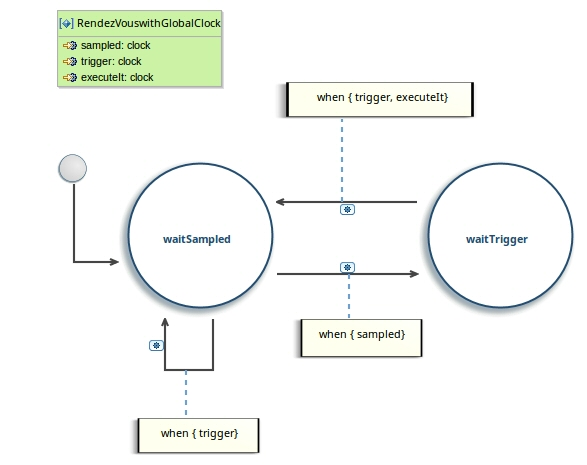
\includegraphics[width=.7\textwidth]{bcool/figs/moccmllib.jpg}
	\caption{State-based representation of the relation \emph{RendezvousWithGlobalClock}}
	\label{fig:moccmllib}
\end{figure}

By using this event relation, we rewrite the coordination rule as shown in Listing~\ref{lst:bcoolrunningexamplellib}; the FSMEventOccurs is the \emph{sampled} event, the globalClock is the \emph{trigger} event and the ActionExecute is the \emph{executeIt} event. 


\begin{lstlisting}[language=bcool,
caption={\bcool specification of an operator that illustrates the use of a \moccml library},
label={lst:bcoolrunningexamplellib}, 
basicstyle=\scriptsize\ttfamily, backgroundcolor=\color{LGrey}, numbers=left, firstnumber=8, xleftmargin=2pt]
do: 
	RendezVouswithGlobalClock(FSMEventOccurs, globalClock, ActionExecute)
end operator
\end{lstlisting}

Figure~\ref{fig:libvcd} shows the resulting coordination of the models of the coffee machine by using the relation RendezvousWithGlobalClock. In blue, we show the occurrences of the \emph{selectCoffee:occurs} (sampled event) that are sampled by global clock (trigger event). When an occurrence is sampled, this makes the event \emph{selectCoffee:executeIt} (executeIt event) to occur simultaneously with the occurrence of the global clock (in red in Figure~\ref{fig:libvcd}). This represents the sampling of the last occurrence of the event \emph{selectCoffee:occurs}.   
  
\begin{figure}[h]
	\center
	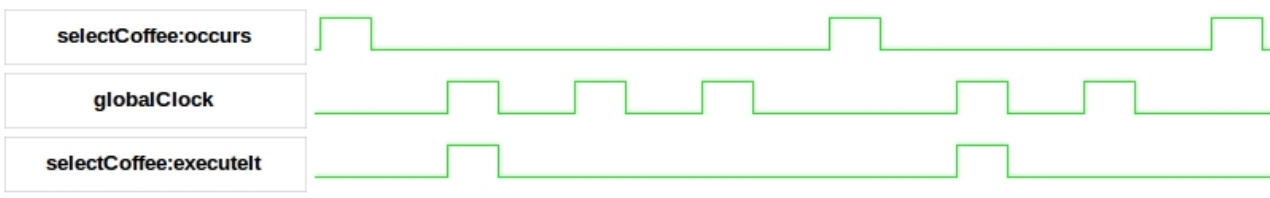
\includegraphics[width=.9\textwidth]{bcool/figs/libvcd}
	\caption{Resulting coordination of the Coffee Machine by using the automata relation \emph{RendezvousWithGlobalClock}}
	\label{fig:libvcd}
\end{figure}


%Listing~\ref{lst:moccmllib} shows a partial representation of the \moccml library \emph{facilities.moccmllib} that provides all the declarations used in the previous examples. Lines 2 and 3 imports \ccsl libraries that contains the declaration of the kernel relations and expression from \ccsl. 

%However, an integrator may need to extend the current library to define new specific constraints depending on its problems and domain. 

%To do so, we use \moccml to define a new event relation named \emph{RendezvousWithGlobalClock} (Listing~\ref{lst:moccmllib}: line 10) that accepts three events as parameter: \emph{ActionExecuting}, \emph{FSMEventTriggering} and \emph{globalClock}. Roughly speaking, the relation synchronizes the events ActionExecuting and FSMEventTriggering by relying on the ticking of globalClock. Then, the coordination rule can be rewritten as shown in Listing~\ref{lst:bcoolrunningexamplellib}. The order of the parameters corresponds with the order of the parameters in the declaration (Listing~\ref{lst:moccmllib}: line 10). 

Libraries enable integrators to organize all relevant event relations and expressions by modeling domains. This improves the readability of a \bcool specification by gathering domain specific relations, which can be reused in other specification. By relying on a \moccml library, the application of \bcool operators results in a \ccsl specification. We can use \ccsl tool (\eg TimeSquare\cite{timesquarebib}) to analyze and execute the generated coordination model. In the next subsection, we further explain how the coordination model is generated from a \bcool specification by presenting the semantics of \bcool.   



%We could also use another language to build the semantics of coordination rules and then take benefit from other analysis tools. In the following section, we present the semantics of \bcool by showing how the generation of a model of coordination is done from a \bcool specification. 

%Libraries enable integrators to organize all relevant event relations and expressions by modeling domains. This improves the readability of a \bcool specification by gathering domain specific relations, which can be reused in other specification.
	
%Event expressions create a new event from their parameters (\eg building the \textit{Union}, or the \textit{Intersection} of its parameters).%Relations, however, constrain the evolution of events given as actual parameters. 
%By relying on \moccml, the application of \bcool operators generate a coordination specification in \ccsl. We can then use \ccsl tool (TimeSquare~\cite{timesquarebib}) to perform analyze and execute the generated coordination specification. This is further discussed in Section~\ref{sec:validation}.

%\begin{lstlisting}[language=moccml,
%		caption={Facilities Library in \moccml},
%		label={lst:moccmllib}, 
%		basicstyle=\scriptsize\ttfamily, backgroundcolor=\color{LGrey}, numbers=left, xleftmargin=2pt]
%		AutomataConstraintLibrary Facilities{ 
%		import "platform:/plugin/fr.inria.aoste.timesquare.ccslkernel.model/ccsllibrary/kernel.ccslLib" as kernel;
%		import "platform:/plugin/fr.inria.aoste.timesquare.ccslkernel.model/ccsllibrary/CCSL.ccslLib" as CCSLLib;
%		RelationLibrary CCSLBasedBCOoLRelations {
%		RelationDefinition RendezVouswithGlobalClockDef[RendezVouswithGlobalClock]{ 
%			Expression sampledActionExecuting = SampledOn (Sampled -> globalClock, Trigger-> ActionExecuting)
%			Expression sampledOccurs = SampledOn (Sampled -> globalClock, Trigger-> FSMEventTriggering)
%			Relation RendezVousSamples[Coincides](Clock2-> sampledActionExecuting , Clock1->FSMEventTriggering)
%		}
%		RelationDeclaration RendezVouswithGlobalClock (ActionExecuting: clock , FSMEventTriggering: clock, globalClock: clock)
%		}
%		}
%\end{lstlisting}